\chapter{GPU Acceleration of FHI-aims}
\label{Sex:appendix_gpu_acceleration}

\section{Introduction}

\subsection{Overview of GPU Acceleration Philosophy in FHI-aims}

FHI-aims uses a batch integration scheme\cite{Havu08} in which the real-space integration points are broken up into spacially localized batches of points. Each batch of points is assigned to an MPI rank, and each MPI rank processes its assigned batches sequentially. After all batches have been processed, the MPI ranks communicate the final results to one another.

The batch integration scheme is at the heart of FHI-aims' O(N) scaling in number of atoms for most of the steps of the SCF cycle. (An important exception is the solution of the Kohn-Sham equations, which will be addressed in the near future.) Only basis elements that touch an integration point will contribute to the quantity being calculated for a given batch. As basis elements have finite spacial extent, for a sufficiently large non-periodic system or unit cell of a periodic system, the number of basis elements needed for a given fixed-sized batch will be saturated. Adding more atoms to the system, i.e. increasing the size of a non-periodic system or using a larger unit cell for a periodic system, will increase the number of batches linearly, but not the work done per batch, leading to linear scaling in number of atoms.

By a happy accident, the batch integration scheme in FHI-aims lends itself naturally to GPU acceleration. The details vary based on the task being accelerated, but the general strategy is:
\begin{enumerate}
\item The MPI rank sets up a batch.
\item The MPI rank communicates batch details to its assigned GPU.
\item The GPU performs work on the batch.
\item If the MPI rank needs to process the batch further, the GPU communicates the results back to its assigned MPI rank.
\item After all batches have been processed, the GPU communicates its final results back to its assigned MPI rank.
\end{enumerate}

As each MPI rank processes its batch independent of other MPI ranks, no significant effort is needed to use GPU acceleration in an MPI environment. The batches are small enough that they fit into memory on an NVIDIA GPU. As each batch is statistically similar in size, the memory usage of a given batch is independent of system size; the GPU will not run out of memory as the system size increases for a fixed number of MPI ranks. Furthermore, most of the computation time for tasks utilizing the batch integration scheme is taken up by a small number of BLAS/LAPACK subroutine calls occurring at the end of the batch processing. These subroutine calls can be easily replaced by cuBLAS (\url{https://developer.nvidia.com/cublas}) calls.

The pseudocode for this process is:
\begin{verbatim}
  do i_batch = 1, n_batches
    set_up_batch_on_cpu
    copy_batch_information_to_gpu
    call cuBLAS_Function()
    if gpu_data_needed_on_cpu
      copy_partial_gpu_data_back_to_cpu
      cpu_performs_work_on_partial_gpu_data
    end if
  end do

  copy_gpu_final_data_back_to_cpu
\end{verbatim}

\subsection{Current State of GPU Acceleration in FHI-aims}

The steps needs to use GPU acceleration in FHI-aims are:
\begin{enumerate}
\item Make sure prerequisites are installed.
\item Compile FHI-aims with GPU support. This may be accomplished by using CMake or Makefile.
\item Add GPU acceleration keywords to \texttt{control.in}.
\item Run FHI-aims as normal.
\end{enumerate}

It cannot be stressed enough that the user should consult the documentation for their architecture, as their architecture may require additional steps to use GPU acceleration beyond what is listed here.

The GPU acceleration code is considered stable and suitable for production calculations. An example scaling plot for timings of the first SCF step for 128 atoms of GaAs on Titan Cray XK7 is shown in Figure \ref{fig:GPU_Scaling}. We generally find that the charge density update shows the largest GPU acceleration speed-up.

Larger speed-ups are observed as the basis set size is increased. If a non-periodic system or unit cell of a periodic system is too small (say, a primitive cell of GaAs running on 32 MPI ranks), a slow-down may actually be observed.

\begin{figure}
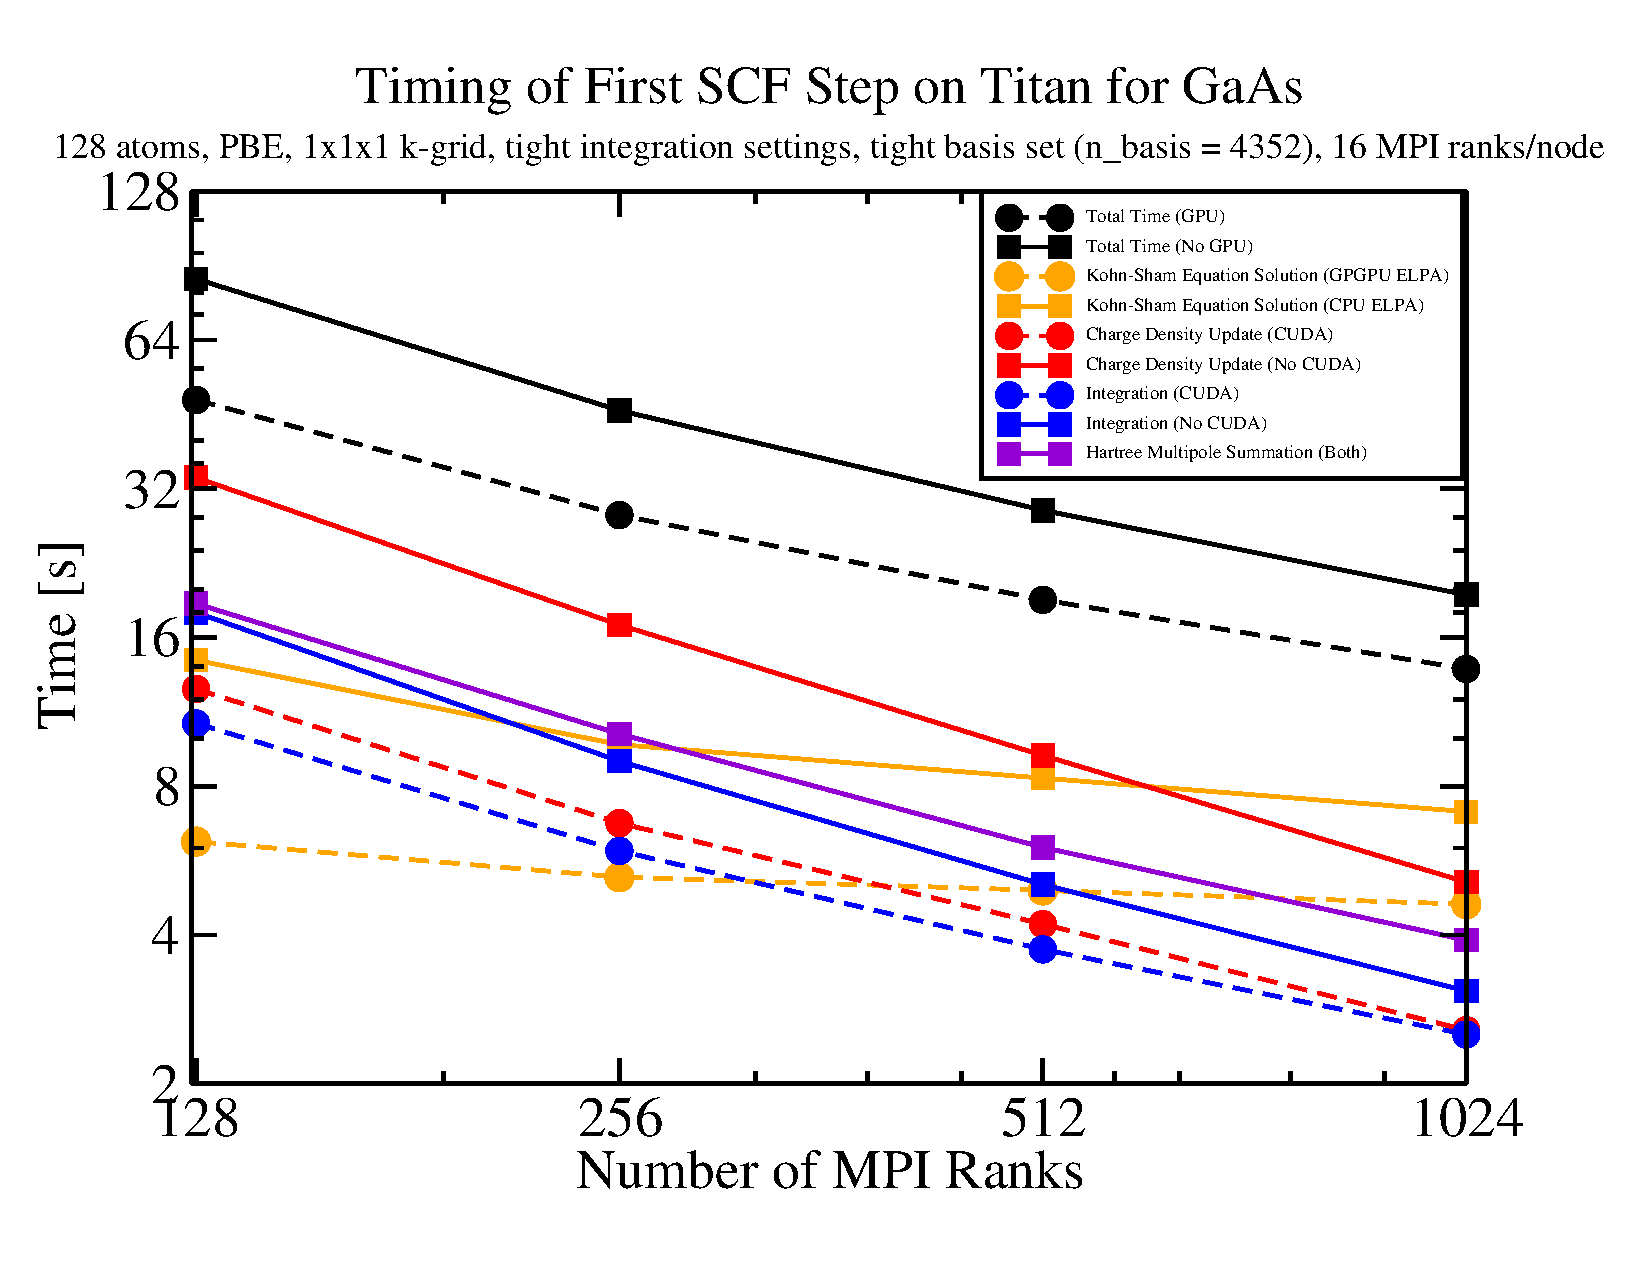
\includegraphics[width=\linewidth]{GaAs_4x4x4Supercell_NoPrecond_GPUBatchSize200}
\caption{Example scaling plot for GPU acceleration. The solid lines are CPU-only calculations, and the dotted lines are GPU-accelerated calculations. At present, there is no GPU acceleration in the Hartree multipole summation, so both CPU-only and GPU-accelerated calculations have the same timings for this task.}
\label{fig:GPU_Scaling}
\end{figure}

The list of tasks we have GPU accelerated natively in FHI-aims is:
\begin{itemize}
\item Integration of the Hamiltonian matrix
\item Charge density update via density matrices
\item Pulay forces
\item Stress tensor
\end{itemize}

In the future, we plan to natively GPU accelerate the following tasks:
\begin{itemize}
\item Hartree multipole summation
\item Construction of the Fock matrix (for Hartree-Fock, hybrid-functional, and beyond)
\end{itemize}

\section{Prerequisites}
The CUDA Toolkit package is needed to enable GPU acceleration in FHI-aims. Supplied by NVIDIA, CUDA may be downloaded free of charge at \url{https://developer.nvidia.com/cuda-toolkit}. It is recommended to use the NVIDIA Multi-Process Service (MPS, see \url{https://docs.nvidia.com/deploy/pdf/CUDA_Multi_Process_Service_Overview.pdf}).

The bulk of the testing of the GPU acceleration code was performed with CUDA 7.5, but code development and early testing used CUDA versions ranging from 5.5 to 10.1. We anticipate that the GPU acceleration in FHI-aims should continue to work with these and future CUDA versions.

\section{Installation}
Compiling the FHI-aims executable with support for GPU acceleration requires a set of GPU acceleration flags be included in the CMake initial cache file. The installation procedure is otherwise the same as a standard FHI-aims installation. We have only tested the GPU code for the scalapack.mpi target, but it should work for any target.

\subsection{Example \texttt{initial\_cache.cmake} file for GPU Acceleration}

\textbf{Note} The example below, created for `node18` of the Timewarp cluster at Duke university, covers the GPU-related flags in \texttt{initial\_cache.cmake}. It may be used as a template for the user's \texttt{initial\_cache.cmake}. We encourage users to put their own GPU acceleration compilation flags on the ``Known compiler settings'' section of the FHI-aims GitLab wiki (\url{https://aims-git.rz-berlin.mpg.de/aims/FHIaims/wikis}).

Architecture of Timewarp `node18`:
\begin{itemize}
\item CentOS Linux 7
\item Intel Xeon Silver 4114 CPU 2.20GHz
\item NVIDIA Titan V100
\item Intel Fortran 18.0.2
\item CUDA 10.1
\item CMake 3.15.4 (some flags below are technically not needed for CMake 3.8+)
\end{itemize}

\texttt{initial\_cache.cmake}:
\begin{verbatim}
set(CMAKE_C_COMPILER icc CACHE STRING "")
set(CMAKE_C_FLAGS "-O3 -ip -fp-model precise -DNDEBUG" CACHE STRING "")
set(CMAKE_CXX_COMPILER icpc CACHE STRING "")
set(CMAKE_CXX_FLAGS "-O3 -ip -fp-model precise -DNDEBUG" CACHE STRING "")
set(CMAKE_Fortran_COMPILER mpiifort CACHE STRING "")
set(CMAKE_Fortran_FLAGS "-O3 -ip -fp-model precise" CACHE STRING "")
set(Fortran_MIN_FLAGS "-O0 -fp-model precise" CACHE STRING "")

set(USE_CUDA ON CACHE BOOL "")
set(CMAKE_CUDA_COMPILER nvcc CACHE STRING "")
set(CMAKE_CUDA_FLAGS "-O3 -DAdd_ -arch=sm_70" CACHE STRING "")

set(LIB_PATHS "$ENV{MKLROOT}/lib/intel64 $ENV{CUDA_HOME}/lib64" CACHE STRING "")
set(LIBS "cublas cudart mkl_scalapack_lp64 mkl_blacs_intelmpi_lp64
    mkl_intel_lp64 mkl_sequential mkl_core" CACHE STRING "")
\end{verbatim}

\begin{itemize}
\item How to determine the \texttt{-arch} or \texttt{-gencode} CUDA flags? Your CUDA installation should come with a utility called deviceQuery, which is located in \\
\texttt{samples/1\_Utilities/deviceQuery} in the CUDA root directory. Copy that directory into your work directory, enter, and build. If you get any build errors, edit the Makefile accordingly. When successful, run the executable \texttt{deviceQuery}. The line ``CUDA Capability Major/Minor version number'' contains the relevant information. For example, if it says 6.0 then use \texttt{sm\_60} with the \texttt{-arch} or \texttt{-gencode} flags.
\item How to choose between multiple GPU cards installed on the system? Use the environment variable \texttt{CUDA\_VISIBLE\_DEVICES}.
\item With CMake version $<3.8$, the CUDA libraries need to be linked manually. If unsure, try including ``cublas cudart'' in \texttt{LIBS} and edit \texttt{LIB\_PATHS} accordingly.
\item When using the GNU Fortran compiler with CMake version $\ge3.8$ and $<3.11$, it can happen that the executable wants to link to the wrong libgfortran library at runtime. This can be prevented by pointing \texttt{CUDA\_LINK\_DIRS} to directories that contain the CUDA libraries (e.g., ``/opt/cuda/lib64/stubs /opt/cuda/lib64''). For more information, see this: \url{gitlab.kitware.com/cmake/cmake/issues/17792}.
\end{itemize}

\section{Running FHI-aims with GPU Acceleration}
Compiling the FHI-aims executable with GPU acceleration support will not automatically turn on GPU acceleration. To use GPU acceleration when running FHI-aims, the user specifies which tasks should be GPU accelerated independently using the \texttt{control.in} keywords below:

\keydefinition{use\_gpu}{control.in}
{
  \noindent
  Usage: \keyword{use\_gpu} \\[1.0ex]
  Purpose: Use GPU acceleration methods that are considered stable. This keyword currently enables \keyword{gpu\_density}, \keyword{gpu\_hamiltonian}, and \keyword{gpu\_pulay}. These keywords can also be used individually to turn on GPU acceleration in a specific part of FHI-aims.
}

\keydefinition{gpu\_density}{control.in}
{
  \noindent
  Usage: \keyword{gpu\_density} \\[1.0ex]
  Purpose: Use GPU acceleration when updating the charge density via density matrices. This keyword does nothing when using orbital-based density update. \\[1.0ex]
}

\keydefinition{gpu\_hamiltonian}{control.in}
{
  \noindent
  Usage: \keyword{gpu\_hamiltonian} \\[1.0ex]
  Purpose: Use GPU acceleration when integrating the Hamiltonian matrix. \\[1.0ex]
}

\keydefinition{gpu\_pulay}{control.in}
{
  \noindent
  Usage: \keyword{gpu\_pulay} \\[1.0ex]
  Purpose: Use GPU acceleration when calculating the Pulay forces and analytical stress tensor. \\[1.0ex]
}

One important keyword when running GPU-accelerated calculations is \keyword{points\_in\_batch}, which sets the targeted number of points per batch. This parameter is a trade-off: increasing the number of points per batch increases the work done by the GPU per batch, increasing the efficiency of the GPU, but it also increases the number of basis elements interacting with a batch, increasing the memory usage. Due to technical details, some of this additional work is unnecessary, as it does not appreciably add to the integrals being evaluated.

The default value for \keyword{points\_in\_batch} based on early CPU-only benchmarks was set to 100. We have found that increasing this value to 200 is a better choice for our test architecture (Kepler Tesla GPUs) when using GPU acceleration, and we have set 200 as the default value when running any GPU-accelerating any tasks involving the batch integration scheme. The user should also play around with this parameter for their own architecture, particularly if they are using a different GPU architecture.

All GPU keywords may be set independently. We have found that the charge density update shows a significantly higher GPU-accelerated speed-up than the Hamiltonian integration (c.f. Figure \ref{fig:GPU_Scaling}). If the user's architecture uses fast CPUs but slow GPUs, enabling GPU acceleration for the Hamiltonian integration may actually slow down the calculation.

\subsection{Memory Usage with GPU Acceleration}

One hypothetical limitation in the current implementation of GPU acceleration in FHI-aims is GPU memory usage. All MPI ranks are assigned to one of the available GPUs, implying that a GPU will generally have more than one MPI rank assigned to it. All MPI ranks will offload their work during the compute-intensive cuBLAS call onto the assigned GPU. This creates two bottlenecks: not only do MPI ranks need to ``wait their turn'' behind other MPI ranks before the GPU processes their current batch, but each MPI rank will take up a portion of the GPU's memory. If a calculation runs out of memory when using GPU acceleration, some possible solutions are:
\begin{itemize}
\item Reduce the basis set density, if possible. This should only be done if additional basis set elements were uncommented in the species defaults; we do not recommend the user uses less basis elements than the default ``tight'' basis set unless they know exactly what they're doing.
\item Read Section \ref{Sec:Large-scale}, ``Large-scale, massively parallel: Memory use, sparsity, communication, etc.'' of the manual. In particular, consider setting \keyword{use\_local\_index} to \texttt{.true.} . While there will be a time cost associated with enabling this keyword, the memory savings can be considerable.
\item Use less MPI ranks per node. By having less MPI ranks per node, less MPI ranks will be bound to the GPUs on each node, reducing the overall GPU memory usage.
\end{itemize}

\subsection*{Summary}
\begin{itemize}
\item Use keywords in \texttt{control.in} to enable GPU acceleration. \item Optimize \keyword{points\_in\_batch} for the architecture used.
\item Test each GPU acceleration keyword individually to make sure there is a speed up compared to the CPU-only version for the architecture used.
\item Reduce the basis set size or set \keyword{use\_local\_index} to \texttt{.true.} if your calculation runs out of memory. (This is true for all calculations, not just GPU-accelerated calculations.)
\end{itemize}
